%!TEX root = ../main.tex

\noindent 
Στο κεφάλαιο αυτό αναφέρονται οι θεωρητικές έννοιες πάνω στις οποίες στηρίζεται η συγκεκριμένη εργασία. Αρχικά αναλύεται η διαδικασία της στερεοφωνικής και αμφιωτικής ακρόασης, η συνάρτηση μεταφοράς του κεφαλιού καθώς και η έννοια της αμφιωτικής κρουστικής απόκρισης δωματίου. Στη συνέχεια περιγράφονται οι διωτικές παράμετροι, ILD και ITD, καθώς και το μοντέλο του Dietz \cite{Dietz2011} το οποίο εφαρμόστηκε για την εξαγωγή τους και η έννοια του λευκού θορύβου. Στη συνέχεια προσεγγίζονται οι απαραίτητες έννοιες της μηχανικής μάθησης όπως και οι δομές των νευρωνικών που εκπαιδεύτηκαν, τα στοιχεία από τα οποία αυτές αποτελούνται, οι μετρικές αξιολόγησής τους και η σημασία της επιλογής ενός κατάλληλου βελτιστοποιητή (optimizer) στην ταχύτητα σύγκλισης του εκάστοτε μοντέλου.

\section{Στερεοφωνική και Αμφιωτική ακρόαση}

Σε αυτή την ενότητα δίνονται οι βασικές αρχές που διέπουν την αντιληπτική λειτουργία εντοπισμού της θέσης ακουστικών πηγών στο χώρο και οι σχετικές τεχνολογικές προσεγγίσεις που ακολουθούνται από τα ηχητικά συστήματα.

\subsection{Στερεοφωνική ακρόαση}

Ο πλέον διαδεδομένος τρόπος αναπαραγωγής του ήχου για οικιακή ή ατομική ακρόαση είναι η στερεοφωνία που βασίζεται στη χρήση δύο ανεξάρτητων καναλιών (αριστερού-L και δεξιού-R) στα οποία συνδυάζονται πολλαπλά κανάλια και πηγές κατά την ηχογράφηση και τα οποία αναπαράγονται από δύο ηχεία, κατάλληλα τοποθετημένα στο χώρο και σε σχέση με τον ακροατή ή και από ακουστικά κυρίως για ακρόαση από φορητές συσκευές.

Σε ακρόαση με φυσικό τρόπο, η αντίληψη που δημιουργείται από την ύπαρξη μιας ακουστικής πηγής στο ελεύθερο ακουστικό πεδίο ή και χώρο, οφείλεται στα συνδυασμένα ερεθίσματα από τα δύο αυτιά του ακροατή που επιτρέπουν τον προσδιορισμό της θέσης της πηγής. Η λειτουργία του μηχανισμού χωρικής αντίληψης του ήχου στηρίζεται εν πολλοίς στην αποκαλούμενη \textit{\textbf{δυϊκή θεωρία}} (duplex theory). Σύμφωνα με τη θεωρία αυτή, το κάθε αυτί, λόγω της διαφορετικής απόστασής του από την ηχητική πηγή $d_1$ και $d_2$ όπως φαίνεται στο Σχήμα \ref{fig:stereo_listening_mechanism}, λαμβάνει διαφορετικές τιμές ηχητικής πίεσης $p_L(t)$ και $p_R(t)$ λόγω:
\begin{enumerate}
    \item Της εξασθένησης της τιμής της πίεσης συναρτήσει της απόστασης.
    \item Της διαφοράς φάσης ή και σχετικής καθυστέρησης λόγω του διαφορετικού χρόνου άφιξης του ήχου σε κάθε αυτί.
    \item Της πρόσθετης εξασθένησης που δημιουργείται στην ακουστική πίεση στο αυτί που 'καλύπτεται' ακουστικά από το κεφάλι, που δημιουργεί σε περιοχή των συχνοτήτων φαινόμενα ηχητικής σκίασης.
\end{enumerate}{}

Αναλόγως με τη συχνότητα, το ποιος από τους παραπάνω λόγους είναι σημαντικότερος για την εξασθένιση και αναλύεται περαιτέρω στην ενότητα \ref{sec:binaural_cues}, αλλά γενικότερα οι παραπάνω μηχανισμοί λειτουργούν επί το πλείστον συμπληρωματικά.

\begin{figure}[h]
  \centering
  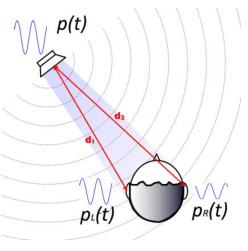
\includegraphics[width=6cm, height=6cm]{images/stereo_listening_mechanism.png}
  \caption{Απεικόνιση του μηχανισμού στερεοφωνικής ακρόασης}
  \label{fig:stereo_listening_mechanism}
\end{figure}

Οι ακροατές εντοπίζουν και διαφοροποιούν με ακρίβεια πηγές που δεν εμφανίζουν σχετικές διαφορές ηχοστάθμης ή/και φάσης στα δύο αυτιά (πχ μια πηγή που είναι ακριβώς μπροστά από το παρατηρητή και μια που είναι ακριβώς από πίσω του στην ίδια απόσταση), στην αντίληψη αξιοποιούνται επιπλέον φαινόμενα ανακλάσεων από τον άνω κορμό (ώμος, στήθος κλπ.) καθώς επίσης και την επίδραση του εξωτερικού πτερυγίου του αυτιού που συλλέγει και διαφοροποιεί τα ηχητικά κύματα που φτάνουν σε αυτό ανάλογα με τις διαφορετικές γωνίες πρόσπτωσης και στα δύο επίπεδα.

\subsection{Αμφιωτική ακρόαση}

Ο άνθρωπος ως ακουστικός δέκτης παρουσιάζει εξαιρετικές ικανότητες στην αναγνώριση και εντοπισμό ηχητικών πηγών στον τρισδιάστατο χώρο. Οι βασικές αρχές αντίληψης της θέσης των πηγών στον τρισδιάστατο χώρο που προαναφέρθηκαν και αφορούν τις σχετικές στάθμες, χρόνους άφιξης ενός σήματος στα 2 αυτιά, της σκίασης του κεφαλιού, της ως προς την γωνία φιλτραρίσματος του σήματος από το πτερύγιο του αυτιού και από τις ανακλάσεις στον άνω κορμό, μπορούν να γενικευθούν σε ένα πλαίσιο που συμπεριλαμβάνει όλους αυτούς τους καθοριστικούς μηχανισμούς και μπορούν να περιγράψουν την αμφιωτική ακρόαση.

Κατά τη γενική περίπτωση αμφιωτικής ακρόασης μιας ακουστικής πηγής, ο ήχος που φτάνει στα δύο αυτιά του ακροατή έχει σαν αποτέλεσμα την αντίληψη και τον προσδιορισμό της θέσης της πηγής σε κάποια γωνία τόσο στο οριζόντιο, όσο και στο κάθετο επίπεδο καθώς και την απόσταση που βρίσκεται αυτή (Σχήμα \ref{fig:binaural_perception_acoustic_source}). Η ικανότητα αυτή προκύπτει από την αντιληπτική διαδικασία που αξιοποιεί τη διαφοροποίηση των σημάτων που φτάνουν στα δύο αυτιά και είναι χαρακτηριστική τόσο για κάθε γωνία στο κάθετο, όσο και στο οριζόντιο επίπεδο. Η δυνατότητα εντοπισμού, εξαρτάται από την μορφολογία του πτερυγίου, του κεφαλιού και του άνω κορμού του εκάστοτε ακροατή. Η ευκρίνεια προσδιορισμού στο οριζόντιο επίπεδο είναι της τάξης των $5^o$ ενώ στο κάθετο επίπεδο είναι αρκετά χειρότερη.

Για την ανάλυση και την περιγραφή της αντιληπτικής διαδικασίας μέσω της δυϊκής θεωρίας, αξιοποιούνται η Αμφιωτική Διαφορά Στάθμης (ILD) και η Αμφιωτική Διαφορά Χρόνου (ITD) που αναλύονται στην ενότητα \ref{sec:binaural_cues}.

Οι δύο αυτές παράμετροι όμως δεν αρκούν για τον προσδιορισμό της θέσης μιας πηγής. Πρέπει να ληφθεί υπόψιν και η διαμόρφωση που εισάγει το εξωτερικό αυτί μέσω του σχήματος του πτερυγίου. Το προσπίπτον σήμα στο κάθε αυτί διαφοροποιείται και φασματικά, αναλόγως με τη γωνία πρόσπτωσης, λόγω της μορφολογίας του πτερυγίου του αυτιού που είναι χαρακτηριστική για κάθε άνθρωπο. Ο τρόπος που το εξωτερικό αυτί συνδυάζεται (μοντελοποιείται) μαζί με τις αμφιωτικές παραμέτρους που αναφέρθηκαν, αναλύονται στην ενότητα \ref{sec:HRTF}


\begin{figure}[h]
  \centering
  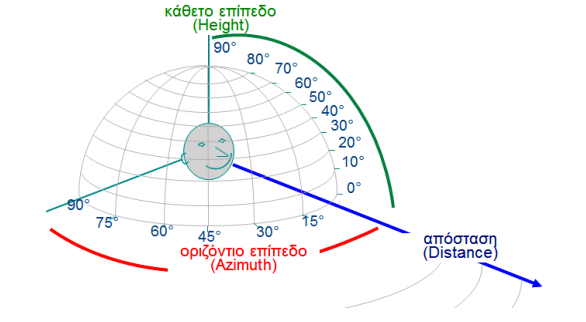
\includegraphics[width=\textwidth]{images/binaural_perception_acoustic_source.png}
  \caption{Αντίληψη και εντοπισμός θέσης πηγής μέσω αμφιωτικής ακρόασης}
  \label{fig:binaural_perception_acoustic_source}
\end{figure}

\section{Συνάρτηση Μεταφοράς Κεφαλιού - HRTF} \label{sec:HRTF}


Η συνάρτηση μεταφοράς του κεφαλιού (Head Related Trasnfer Function - HRTF) είναι μια συνάρτηση μεταφοράς, που για μια συγκεκριμένη γωνία πρόσπτωσης, περιγράφει τη μετάδοση του ήχου από ένα ελεύθερο πεδίο (free field) και την επίδραση του κεφαλιού, του λοβού και του θώρακα σε ένα σημείο στο κανάλι του αυτιού (Σχήμα \ref{fig:auditory_system}) ενός ανθρώπου \cite{mller1995head}. Στο πεδίο του χρόνου η HRTF λέγεται κρουστική απόκριση κεφαλιού (Head Related Impulse Response - HRIR). Η HRIR Παρουσιάζει με έναν εύχρηστο και συνοπτικό τρόπο το ILD και ITD μεταξύ των αυτιών καθώς και άλλες φασματικές πληροφορίες \cite{Enzner2013}.

Στην \cite{doi:10.1121/1.415856}, η συνολική ακουστική μεταφορά από μία ακουστική πηγή σε ελεύθερο χώρο έως το τύμπανο ενός ακροατή, χωρίζεται σε τρία κομμάτια ως εξής:

\begin{itemize}
    \item Μεταφορά από ελεύθερο πεδίο στην φραγμένη είσοδο του ακουστικού καναλιού
    \item Μετατροπή της αντίστασης που σχετίζεται με την φραγή του ακουστικού καναλιού
    \item Μεταφορά μέσω του ακουστικού καναλιού
\end{itemize}{}

\subsection{Μέτρηση HRTF}

Ένα σετ HRTF αριστερού και δεξιού αυτιού εξαρτάται από την θέση της πηγής, την θέση του ακροατή, τη θέση του κεφαλιού και του θώρακα και άλλες παραμέτρους. Οι τυπικές διατάξεις μέτρησης, επιτρέπουν τη μεταβολή ενός ή δύο βαθμών ελευθερίας. Στις περισσότερες περιπτώσεις, μεταβάλλεται η γωνία της πηγής, σε σχέση με το κεφάλι και τον θώρακα που έχουν σταθερό προσανατολισμό. Για την αποτελεσματικότερη μέτρηση HRIR και BRIR (βλ. \ref{sec:BRIR}) έχουν κατασκευαστεί βοηθητικά μοτέρ που επιτρέπουν την περιστροφή ή την αλλαγή της κλίσης του κεφαλιού μέσω λογισμικού, με ακρίβεια μέχρι και $0.01^o$. Συνήθως γίνονται μετρήσεις στο διάστημα $\pm90^o$, με τις $0^ο$ να είναι η πηγή ακριβώς μπροστά από τον δέκτη. Στο Σχήμα \ref{fig:typical-HRTF-measurment-setup} φαίνονται δύο τυπικές διατάξεις μέτρησης HRTF. 

\begin{figure}[h]
  \centering
  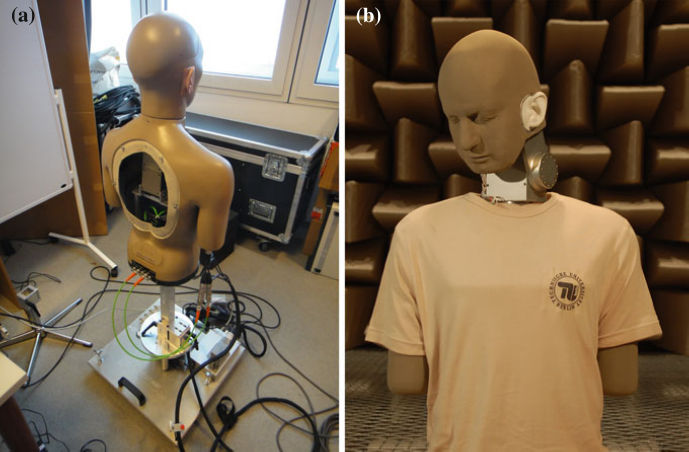
\includegraphics[width=\textwidth]{images/typical-HRTF-measurment-setup.png}
  \caption{Τυπικά σενάρια μέτρησης HRTF: Τροποποιημένο ανδρείκελο KEMAR (a), FABIAN (b)}
  \label{fig:typical-HRTF-measurment-setup}
\end{figure}

\subsection{Υπολογισμός HRTF}

Η επιλογή του σήματος διέγερσης που εκπέμπει η πηγή διαδραματίζει πολύ μεγάλο ρόλο στα αποτελέσματα. Η βέλτιστη διέγερση, εξαρτάται κυρίως από τον αλγόριθμο υπολογισμού της HRIR, αλλά ταυτόχρονα και από το σενάριο μέτρησης (στατικό ή δυναμικό, το περιβάλλον, το υλικό που χρησιμοποιείται κλπ.). Για την επίτευξη ενός υψηλού SNR, το σήμα διέγερσης πρέπει να έχει υψηλή ενέργεια, συγκριτικά με το σύστημα μέτρησης, σε όλη τη συχνοτική περιοχή ενδιαφέροντος. Συχνότερα χρησιμοποιούνται Maximum Length Sequences (MLS), τα οποία είναι περιοδικές ακολουθίες bit που δημιουργούνται από καταχωρητές μετατόπισης γραμμικής ανατροφοδότησης (linear-feedback shift registers) ή απεριοδικά sweep.

Στη συνέχεια, το σήμα αναπαράγεται από το ηχείο-πηγή, και γίνεται συγχρονισμένα η καταγραφή της απόκρισης του αριστερού και δεξιού καναλιού. Η απόκριση συχνότητας προκύπτει από γραμμική αποσυνέλιξη, συνήθως στο πεδίο της συχνότητας. Ένα αποδεκτό SNR για τέτοιου είδους μετρήσεις είναι κάπου ανάμεσα στα 60-90 dB. Μετρήσεις HRTF, πλέον γίνονται και σε ανθρώπους, όχι μόνο σε ανδρείκελα, με ειδικά κατασκευασμένα ακουστικά το περίβλημα των οποίων τυπώνεται με 3Δ εκτυπωτές. 

\subsection{Βάσεις δεδομένων HRTF}

Οι HRTF είναι ένα αναπόσπαστο κομμάτι της τεχνολογίας αμφιωτικής ακοής και ακρόασης. Από την άλλη, η μέτρηση των HRTF είναι ένα δύσκολο και ευαίσθητο εργαστηριακό αντικείμενο. Συνήθως απαιτείται ένας ανηχοϊκός θάλαμος για τη μέτρηση των HRTF, και επιπλέον αρκετός χρόνος από την πλευρά του χειριστή του πειράματος αλλά και του υποκειμένου μέτρησης, ώστε να ολοκληρωθούν οι μετρήσεις με ικανοποιητικό βαθμό χωρικής ανάλυσης. Απαιτούνται ένα ή περισσότερα ηχεία, ακουστικά in-ear, και λογισμικό αναπαραγωγής και καταγραφής ήχου. 

Υπάρχουν αρκετά τέτοια συστήματα, αλλά είναι σαφές πως δεν είναι φορητά. Ως αποτέλεσμα, πολλοί οργανισμοί έχουν επιλέξει να παρέχουν τις μετρήσεις ως δημόσια διαθέσιμες βάσεις δεδομένων στην κοινότητα. Παρακάτω αναφέρονται κάποιες από αυτές. Εκτός αν αναφέρεται διαφορετικά, οι κρουστικές αποκρίσεις παρέχονται με συχνότητα δειγματοληψίας $F_s = 44.1 kHz$.

\begin{itemize}
   \item KEMAR - βάση δεδομένων HRTF από το MIT-Media-Lab \cite{Gardner1995}: Η πρώιμη αυτή βάση δεδομένων είναι ακόμα ιδιαίτερα δημοφιλής, χρησιμοποιώντας το Knowles-Electronics Mannequin for Acoustic Research (KEMAR), αναπαριστά μια εκτενή καταγραφή HRTF. Συνολικά, δειγματοληπτούνται 710 διαφορετικές θέσης, για ανύψωση από $-40^o$ μέχρι $+90^o$ με χωρική ανάλυση $10^o$ στον κάθετο άξονα και περίπου $5^o$ στον οριζόντιο, για απόσταση περίπου 1.4 m μεταξύ του ηχείου και του KEMAR.
   
   \item AUDIS - Ο κατάλογος AUDIS ανθρωπίνων HRTF: Στο γενικό πλαίσιο της Ε.Ε., το project Auditory Displays (AUDIS) \cite{Blauert_1998}, το οποίο βασίστηκε σε μεγάλο βαθμό στην αμφιωτική τεχνολογία και αξιόπιστες HRTF ανθρώπων, πραγματοποιήθηκε ένα ειδικό πρόγραμμα συλλογής HRTF. Εδώ οι συνθήκες μετρήσεων είναι: 2.4 m από το ηχείο, ανάλυση $10^o$ στον κάθετο άξονα από $-10^o$ μέχρι $+90^o$, και ανάλυση $15^o$ στον οριζόντιο άξονα. Οι συνολικές μετρήσεις περιλαμβάνουν 122 κατευθύνσεις για 20 ανθρώπους. Τέθηκε επίσης ένα σύνολο \textit{Golden Rules} για μετρήσεις HRTF.
   
   \item CIPIC - βάση δεδομένων HRTF του εργαστηρίου CIPIC \cite{AlgaziOct.21242001}: Η βάση δεδομένων, περιέχει HRTF μετρημένες με υψηλή χωρική ανάλυση, για περισσότερους από 90 ανθρώπους, με 45 αυτών να είναι δημόσια διαθέσιμοι, συμπεριλαμβανομένου του KEMAR, με μεγάλο και μικρό λοβό. Η χωρική ανάλυση είναι $5^o$ στον κάθετο αλλά και στον οριζόντιο άξονα. Προκύπτουν έτσι 1250 σημεία στην ακουστική σφαίρα 1m, όπου ήταν η απόσταση του ηχείου. Παρέχονται επίσης ανθρωπομετρικά χαρακτηριστικά για κάθε υποκείμενο μέτρησης, καθώς και βοηθητικές συναρτήσεις για το περιβάλλον MATLAB.
   
   \item LISTEN - η βάση δεδομένων HRTF IRCAM: Αναπτηγμένη σε πρότζεκτ της Ε.Ε., περιέχει μετρήσεις HRTF με για  ανύψωση από $-45^o$ μέχρι $+90^o$ με χωρική ανάλυση $5^o$ και περίπου $15^o$ ανάλυση στον οριζόντιο άξονα. Συνολικά μετριούνται 187 θέσεις. Παρέχονται οι μετρήσεις HRTF, προαιρετική διόρθωση diffuse-field και μορφολογικά δεδομένα. Τα δεδομένα που μετρήθηκαν για 50 ανθρώπους είναι διαθέσιμα online\footnote{http://recherche.ircam.fr/equipes/salles/listen/index.html}.
   
   \item ARI - Βάση δεδομένων του Acoustics-Research-Institute: Περιέχει HRTF υψηλής ανάλυσης για πάνω από 70 ανθρώπους. Μετρήθηκαν 1550 θέσεις για κάθε ακροατή, με $2.5^o$ ανάλυση στον οριζόντιο άξονα για γωνίες από $0^o - 359^o$, και ανυψώσεις από $-30^o$ έως $+80^o$. Τα δεδομένα μπορούν να βρεθούν στον σύνδεσμο\footnote{http://www.kfs.oeaw.ac.at/content/view/608/606}.
   
   \item FIU - Βάση δεδομένων HRTF του Florida-International-Univ. DSP-Lab: Μετρήθηκαν 15 διαφορετικά άτομα, για δώδεκα διαφορετικές γωνίες στον οριζόντιο άξονα και έξι στον κάθετο. Παρέχονται 3-Δ εικόνες των λοβών κάθε ατόμου, και ανθρωπομετρικά χαρακτηριστικά. Χρησιμοποιήθηκε συχνότητα δειγματοληψίας $F_s = 96 kHz$ και είναι διαθέσιμη στον σύνδεσμο\footnote{http://dsp.eng.fiu.edu/HRTFDB}.
\end{itemize}

\section{Αμφιωτική Κρουστική Απόκριση Δωματίου - BRIR} \label{sec:BRIR}

Όταν ένας ήχος εκπέμπεται από μια πηγή σε έναν κλειστό χώρο, ένας ακροατής αρχικά θα λάβει τον άμεσο ήχο, ακολουθούμενο από ανακλάσεις από τους τοίχους ή αντικείμενα τοποθετημένα μέσα στο δωμάτιο, όπως φαίνεται στο Σχήμα \ref{fig:listener_reverberant_room}. 

\begin{figure}[h]
  \centering
  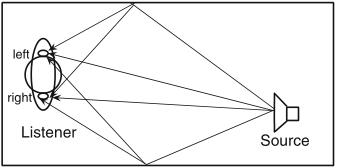
\includegraphics[width=\textwidth]{listener_reverberant_room.png}
  \caption{Ακροατής και ακουστική πηγή σε δωμάτιο με αντήχηση}
  \label{fig:listener_reverberant_room}
\end{figure}

Η ενέργεια του ανακλώμενου ήχου εξασθενεί, σύμφωνα με τα χαρακτηριστικά απορρόφησης των εκάστοτε επιφανειών στο δωμάτιο. Υποθέτοντας ότι η ακουστική του δωματίου, μοντελοποιείται ως ένα \textit{γραμμικό, χρονικά-αμετάβλητο} (ΓΧΑ), σύστημα, η κρουστική απόκριση του δωματίου, (Room Impulse Response - RIR), παρέχει μια πλήρη περιγραφή των άμεσων και ανακλώμενων μονοπατιών από μια πηγή στον δέκτη. Ο χρόνος που χρειάζεται για να ελαττωθεί η ενέργεια του δωματίου κατά 60 dB, αφού η πηγή έχει σταματήσει να εκπέμπει καλείται χρόνος αντήχησης $RT_{60}$ και είναι η παράμετρος που χρησιμοποιείται πιο συχνά για τον προσδιορισμό των ακουστικών ιδιοτήτων ενός δωματίου \cite{Tsilfidis2013}. Σε ένα γενικό, πολυκαναλικό σενάριο, με μία πηγή και \textit{i} δέκτες, το αντιχητικό σήμα $x_i(n)$, μπορεί να εκφραστεί σαν την συνέλιξη του ανηχοϊκού σήματος $s(n)$, με τις αντίστοιχες RIR, $h_i(n)$, ως εξής:

\begin{CEquation}
    x_i(n) = \sum_{j=0}^{J_h - 1} h_i(j)s(n-j) \label{eq 1}
\end{CEquation}

Όπου n αναπαριστά τον δείκτη διακριτού χρόνου και $J_h$ το μήκος της κρουστικής απόκρισης.

Σε ένα αμφιωτικό σενάριο (binaural) η απόκριση του δωματίου, συνδυάζεται με την κρουστική απόκριση του κεφαλιού (Head Related Impulse Response - HRIR), η οποία αποτελείται από δύο κανάλια, ένα για κάθε αυτί. Οι HRIR μετρούνται σε ανηχοϊκές συνθήκες. Συνεπώς, υποθέτοντας μια ιδεατή παντοκατευθυντική πηγή, μία αμφιωτική κρουστική απόκριση δωματίου, για το αριστερό αυτί-κανάλι, $h_L(n)$, μπορεί να εκφραστεί ως

\begin{CEquation}
\begin{split}
    h_L(n) = g(r_s)δ(n-n_s) * h_{\textit{HRIR},L,\theta_d,\phi_d}(n) \\+  \sum_{m=0}^{J_{h_m} - 1} h_{m,L}(n)*h_{\textit{HRIR},L,\theta_m,\phi_m}(n) \label{eq 2}
\end{split}
\end{CEquation}

όπου $g(r_s)$ είναι η ελάτωση του κέρδους που εξαρτάται από την απόσταση πηγής-παρατηρητή $r_s$, $\delta(n)$ η συνάρτηση δέλτα του Kronecker, $n_s$ η καθυστέρηση που εξαρτάται κυρίως από την απόσταση πηγής-παρατηρητή και τα φυσικά χαρακτηριστικά του μέσου διέλευσης. $h_{\textit{HRIR},L,\theta_m,\phi_m}(n)$ είναι η αριστερή HRIR για τον άμεσο ήχο, που αντιστοιχεί σε $\theta_d$ και $\phi_d$, δηλαδή την οριζόντια και κάθετη γωνία μεταξύ του παρατηρητή και της πηγής. Η τιμή $h_m(n)$ αναφέρεται στην m-οστή ανάκλαση. $J_{h_m}$ ο συνολικός αριθμός ανακλάσεων. Τέλος $\theta_m$ and $\phi_m$ είναι οι οριζόντιες και κάθετες γωνίες μεταξύ του δέκτη και της m-οστής ανάκλασης. Αντίστοιχα υπολογίζεται και η BRIR, $h_R(n)$. 

Έτσι, το αντηχητικό σήμα στο αριστερό και δεξί αυτί ενός ακροατή $x_L(n)$ και $x_R(n)$, περιγράφονται με τη συνέλιξη του ανηχοϊκού σήματος $s(n)$, με τις BRIR του αριστερού και δεξιού αυτιού αντίστοιχα, όπως φαίνεται στην Εξίσωση \ref{eq 3}.  Ένα παράδειγμα BRIR από ένα δωμάτιο με ιδιαίτερα υψηλή αντήχηση φαίνεται στο Σχήμα \ref{fig:BRIR_example}

\begin{CEquation}
\begin{split}
    x_L(n) = \sum_{j=0}^{J_{h_L} - 1} h_L(j)s(n-j) \\  \label{eq 3}
    x_R(n) = \sum_{j=0}^{J_{h_R} - 1} h_R(j)s(n-j)
\end{split}
\end{CEquation}

\begin{figure}[H]
  \centering
  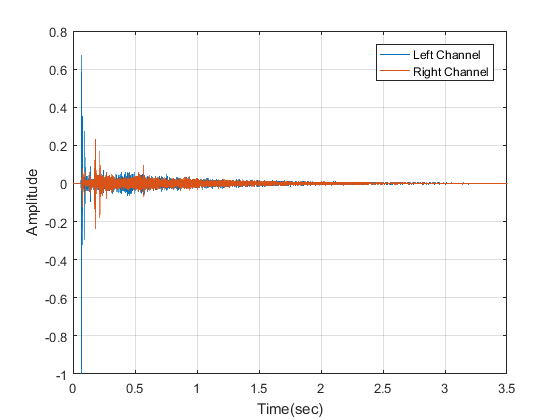
\includegraphics[width=\textwidth]{images/BRIR_example.png}
  \caption{BRIR από δωμάτιο με υψηλή αντίχηση}
  \label{fig:BRIR_example}
\end{figure}

\section{Αμφιωτικές Παράμετροι} \label{sec:binaural_cues}


Το ακουστικό σύστημα, μπορεί να παρομοιαστεί με έναν υπολογιστή πολλαπλών χρήσεων με δύο θύρες εισόδου. Οι θύρες είναι τα δύο αυτιά, στο ίδιο ύψος εκατέρωθεν ενός στερεού ελλειψοειδούς, το κεφάλι.  Το κεφάλι λειτουργεί ως \textit{φορέας μιας κεραίας}, που μπορεί να κινηθεί με έξι βαθμούς ελευθερίας σε σχέση με το σώμα, ενώ το ίδιο το σώμα μπορεί να προηγηθεί στον τρισδιάστατο χώρο, και να αλλάξει τον προσανατολισμό του σε σχέση με τη θέση αναφοράς \cite{Kohlrausch2013}. Μία σύντομη ανατομική περιγραφή του ακουστικού συστήματος φαίνεται στο Σχήμα \ref{fig:auditory_system}

\begin{figure}[h]
  \centering
  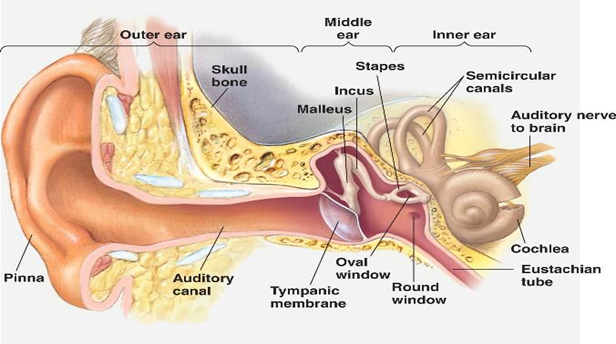
\includegraphics[width=\textwidth]{images/auditory_system.png}
  \caption{Ανατομική περιγραφή του ακουστικού συστήματος}
  \label{fig:auditory_system}
\end{figure}

Το ακουστικό σύστημα δέχεται εισόδους με τη μορφή ελαστικών δονήσεων και κυμάτων, από υγρά ή στερεά με τα οποία είναι σε μηχανική επαφή. Οι είσοδοι έρχονται είτε μέσω του αέρα από τα ακουστικά κανάλια (ear canals) είτε από την μεταβίβαση των οστών μέσω του κρανίου. Συνήθως το κρανίο αγνοείται όταν πρόκειται για ακρόαση σε αέρα, αφού διαφέρει κατά περίπου 60 dB σε σχέση με την μεταβίβαση λόγω αέρα, που αντιστοιχεί σε έναν λόγο ισχύος της τάξεως του $10^6$.

Η ακοή επιτυγχάνεται και με ένα μόνο αυτί, αλλά η ακρόαση με δύο λειτουργικά αυτιά, ή \textit{αμφιωτική ακρόαση}, προσφέρει σημαντικά πλεονεκτήματα έναντι της μονοωτικής ακρόασης. Αυτό, συμβαίνει διότι η αμφιωτική ακρόαση προσφέρει επιπλέον πληροφορία, η οποία κωδικοποιείται στις διαφορές των σημάτων εισόδου στα δύο αυτιά.

Υποθέτοντας ότι αυτές οι διαφορές αναπαρίστανται με ένα γραμμικό, χρονικά αμετάβλητο σύστημα, προκύπτει το συμπέρασμα, ότι μπορούν να υπάρχουν μόνο δύο τέτοιες διαφορές. Η αμφιωτική διαφορά χρόνου άφιξης (Interaural Time Difference - ITD) και οι αμφιωτικές διαφορές έντασης (Interaural Level Difference - ILD). Και οι δύο εξαρτώνται από τη συχνότητα.

Τα υπάρχοντα μοντέλα, αξιοποιούν τις ακουστικές παραμέτρους, που διακρίνονται σε αμφιωτικές παραμέτρους, που είναι πιο εύρωστες και απαιτούν και τα δύο αυτιά για να αναλυθούν, και σε μονοωτικές παραμέτρους που χρειάζονται μόνο το ένα αυτί. Εδώ αναλύονται μόνο οι αμφιωτικές παράμετροι αφού αυτές χρησιμοποιήθηκαν για την προσέγγιση του προβλήματος.

\subsection{Interaural Time Difference}

Παρουσιάζεται πρώτα η ανάλυση του ITD, γιατί ιστορικά το μοντέλο Jefress \cite{Jeffress1948} ήταν το πρώτο μοντέλο εντοπισμού, το 1948. Η βασική ιδέα αυτού του μοντέλου είναι ένας συνδυασμός, \textit{γραμμών καθυστέρησης} και \textit{κυττάρων σύμπτωσης} (coincidence cells). Με βάση το μοντέλο, υπάρχουν δύο ξεχωριστές, παράλληλες γραμμές καθυστέρησης σε κάθε αυτί. Τα σήματα διαδίδονται με αντίθετη κατεύθυνση σε κάθε γραμμή, όπως φαίνεται στο Σχήμα \ref{fig:jeffress-coincidence-mechanism}. Σε κάποιο σημείο, τα σήματα που ταξιδεύουν στις δύο γραμμές, συναντούνται σε ένα κύτταρο σύμπτωσης, το οποίο στέλνει το σήμα στο επόμενο επίπεδο. Λόγω της διαφοράς χρόνου άφιξης των δύο σημάτων στα αυτιά, αυτά θα ενεργοποιήσουν ένα πλευρικά μετατοπισμένο κύτταρο σύμπτωσης, το οποίο κατ' επέκταση αντιστοιχίζεται σε μια πλευρική γωνία άφιξης.

Οι Cherry και Sayers \cite{Cherry1956}, εισήγαγαν τη χρήση της αμφιωτικής ετεροσυσχέτισης, ως μια μέθοδο για την εκτίμηση του ITD η οποία ορίζεται όπως φαίνεται στην Εξίσωση \ref{IACC}. Με την εσωτερική καθυστέρηση να ορίζεται με \textit{τ} και τα αριστερά και δεξιά σήματα πίεσης, $y_l(t)$ και $y_r(t)$. Έχει αποδειχτεί πως αυτό είναι μια καλή προσέγγιση του μοντέλου Jeffress. Το ITD έχει παρατηρηθεί πως δεν παίζει ιδιαίτερο ρόλο στον εντοπισμό πηγών σε συχνότητες μεγαλύτερες των 1500Hz.

\begin{CEquation}
    \psi_{y_{l,r}}(\tau) = \frac{\int_{t=-\infty}^{\infty}y_l(t)y_r(t+\tau)dt}
    {\sqrt{\int_{t=-\infty}^{\infty}y_l^2(t)dt \int_{t=-\infty}^{\infty}y_r^2(t)dt}}
    \label{IACC}
\end{CEquation}

\begin{figure}[h]
  \centering
  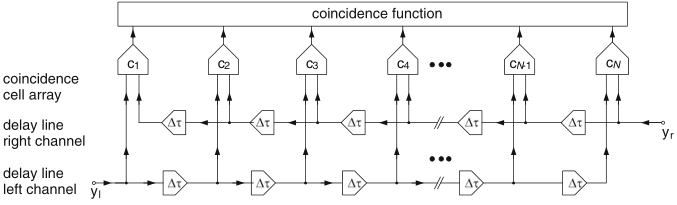
\includegraphics[width=\textwidth]{images/jeffress-coincidence-mechanism.png}
  \caption{Μοντέλο σύμπτωσης όπως αρχικά προτάθηκε από τον Jeffress}
  \label{fig:jeffress-coincidence-mechanism}
\end{figure}

\subsection{Interaural Level Difference}

Οι αμφιωτικές διαφορές έντασης συμβαίνουν λόγω φαινομένων επικάλυψης του κεφαλιού, όταν ένας ήχος φτάνει πλάγια στον δέκτη. Τυπικές τιμές είναι $\pm30 dB$ σε συχνότητες κοντά στα 5 kHz και γωνίες άφιξης στα $\pm60^o$. Στις χαμηλές συχνότητες η επικάλυψη του κεφαλιού δεν παίζει ιδιαίτερο ρόλο, και διαφορές στο ILD σπανίζουν (κάτω από 1500 Hz). Η συχνότητα επικάλυψης ILD και ITD γίνεται φανερό πως είναι στα 1500 Hz.

Το ILD, μπορεί να υπολογιστεί απευθείας από τα σήματα του αριστερού και δεξιού καναλιού όπως φαίνεται στην εξίσωση \ref{ILD_1}, πράγμα το οποίο τυπικά υπολογίζεται για διαφορετικές μπάντες συχνοτήτων, όπου $P_l$ και $P_r$ οι ισχύες των σημάτων που φτάνουν στο αριστερό και δεξί αυτί.
\begin{CEquation}
    \alpha = 10log_{10}(P_l) - 10log_{10}(P_r)
    \label{ILD_1}
\end{CEquation}
Οι Reed και Blum \cite{Reed1990} εισήγαγαν έναν φυσιολογικό (physiological) αλγόριθμο για τον υπολογισμό του ILD, βασισμένο στην δραστηριότητα, $E(\alpha)$, μιας συστοιχίας \textit{El cells}, όπως φαίνεται στο σχήμα \ref{fig:el-cell-structure} και περιγράφεται στην Εξίσωση \ref{eq:reed-and-blum}. Η απόκριση κάθε El-cell είναι συντονισμένη για ένα συγκεκριμένο ILD, και ελατώνεται όσο πιο μακριά από αυτό είναι το ILD των σημάτων άφιξης.

\begin{CEquation}
    E(\alpha) = \exp{
    (10^{\alpha \slash ILD_{max}}\sqrt{P_l} - 
    10^{\alpha \slash ILD_{max}}\sqrt{P_r}})^2
    \label{eq:reed-and-blum}
\end{CEquation}

\begin{figure}[h]
  \centering
  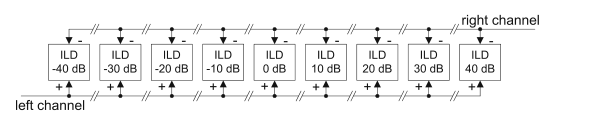
\includegraphics[width=\textwidth]{images/el-cell-structure.png}
  \caption{Δομή El-cell}
  \label{fig:el-cell-structure}
\end{figure}

\subsection{Εντοπισμός ηχητικών γεγονότων}

Υπάρχουν πολλές μέθοδοι για τον υπολογισμό της θέσης ηχητικών πηγών από τις αμφιωτικές παραμέτρους. Μια μέθοδος που επιτυγχάνει αυτόν τον σκοπό, είναι η κατασκευή μια βάσης δεδομένων, που αντιστοιχίζει μετρηθείσες παραμέτρους ILD και ITD σε σφαιρικές συντεταγμένες.

Είναι ακόμα ασαφές πως το ακουστικό σύστημα συνδυάζει τις παραμέτρους για την εξαγωγή συμπερασμάτων για την θέση ακουστικών γεγονότων, συγκεκριμένα, αναπάντητα είναι ακόμα τα εξής ερωτήματα:


\begin{itemize}
    \item Ο τρόπος που συνδυάζονται τα ILD και ITD.
    \item Η ολοκλήρωση της πληροφορίας ως προς τον χρόνο.
    \item Η ολοκλήρωση της πληροφορίας ως προς τη συχνότητα.
    \item Ο διαχωρισμός διαφορετικών, ταυτόχρονων πηγών.
    \item Η αντιμετώπιση των ανακλάσεων του δωματίου.
\end{itemize}

Ότι είναι γνωστό μέχρι στιγμής για τον τρόπο που το ακουστικό σύστημα συνδυάζει τις παραμέτρους έχει προκύψει πειραματικά, από τα αποκαλούμενα trading πειράματα, όπου το ILD υποδεικνύει μια κατεύθυνση, αλλά το ITD μια διαφορετική και ο δέκτης καλείται να κρίνει την πραγματική.

Πιστεύεται ότι το ακουστικό σύστημα, εφαρμόζει χρονικό ή/και συχνοτικό cue weighting, δηλαδή δίνει μεγαλύτερη βαρύτητα σε κάποιες παραμέτρους όταν πληρούνται κάποιες συνθήκες, αλλά ο ακριβής τρόπος που αυτό συμβαίνει είναι ακόμα υπό διερεύνηση. Υπάρχουν διαφορετικές απόψεις, με την μία, που είναι και η επικρατέστερη, να λέει πως το ακουστικό σύστημα δίνει έμφαση στο onset τμήμα του σήματος, ενώ η άλλη να ισχυρίζεται πως ολοκληρώνει την πληροφορία σε μεγαλύτερο χρονικό διάστημα. Τα πράγματα γίνονται σημαντικά δυσκολότερα, όταν δεν είναι σαφές πόσες πηγές υπάρχουν. Τότε οι παράμετροι εκτός από την ανάθεση βαρών σε αυτές, πρέπει να αντιστοιχηθούν και στη σωστή πηγή. Η μεγαλύτερη πρόκληση όμως παραμένει διερεύνηση της αντιμετώπισης των ανακλάσεων του δωματίου από το ακουστικό σύστημα.

\section{Μοντέλο dietz2011} \label{sec:dietz_theory}

Οι Dietz et al. κατασκεύασαν ένα μοντέλο της ανθρώπινης ακοής, με στόχο τον εντοπισμό της κατεύθυνσης ταυτόχρονων ομιλητών στο \cite{Dietz2011}. Ο άνθρωπος έχει μια ιδιαίτερα εύρωστη ικανότητα να εντοπίζει ήχους σε αντίξοες συνθήκες (αντήχηση, έντονος θόρυβος κλπ) οπότε κρίθηκε αναγκαίο να δημιουργηθεί ένα μοντέλο που προσομοιάζει τα χαρακτηριστικά του ανθρώπινου ακουστικού συστήματος με στόχο να χρησιμοποιηθεί αυτό σε αυτόματα συστήματα προσέγγισης DOA.

Η δομή του μοντέλου που κατασκευάστηκε χωρίζεται σε τρία μέρη. Το πρώτο κομμάτι, που θα απασχολήσει αυτή την ενότητα, είναι η ακουστική επεξεργασία για την εξαγωγή των ακουστικών παραμέτρων. Στο δεύτερο, εξάγονται τα σημαντικά τμήματα αυτών των παραμέτρων και στο τρίτο υλοποιείται το σύστημα εντοπισμού. 

\subsection{Ακουστική επεξεργασία}

Εδώ χρησιμοποιήθηκε το μοντέλο ακουστικής επεξεργασίας Interaural Phase Difference \cite{Dietz_2008}, και περιγράφεται παρακάτω.

\begin{enumerate}
    \item Προσεγγίζεται η χαρακτηριστική μεταφοράς του μέσου αυτιού (βλ. \ref{fig:auditory_system}), με ένα πρώτης τάξεως ζωνοπερατό φίλτρο $F_p = 500 Hz, F_c = 2 kHZ$.
    \item Το ακουστικό ζωνοπερατό φιλτράρισμα στην basilar μεμβράνη μοντελοποιείται με μια γραμμική, 4ης τάξης, τράπεζα φίλτρων που αποτελούνται μόνο από πόλους (gammatone filter-bank). Το πλάτος κάθε φίλτρου ορίζεται ως το ισοδύναμο τετραγωνικό εύρως ζώνης (Equivalent Rectangular Bandwidth - ERB) των ακουστικών φίλτρων. Υλοποιούνται 23 μπάντες φίλτρων στο διάστημα των 200 Hz - 5 kHz με απόσταση 1 ERB. Σημειώνεται πως το ERB είναι ένα μέτρο που χρησιμοποιείται στην ψυχοακουστική και δίνει μια εκτίμηση του εύρους ζώνης των φίλτρων στην ανθρώπινη ακοή, χρησιμοποιώντας μη ρεαλιστικά, αλλά βολικά μοντέλα τετραγωνικών ζωνοπερατών φίλτρων.
    \item Η συμπίεση του κοχλία λογιστικοποιήθηκε με άμεση συμπίεση ισχύος 0.4, μετά το bandpass φιλτράρισμα.
    \item Η διαδικασία της ηλεκτρομηχανικής μεταγωγής των εσωτερικών hair-cells, προσομοιώνεται με την ανόρθωση ημίσεος κύματος με διαδοχικά lowpass φίλτρα 5ης τάξης με $F_c = 770 Hz$.
    \item Οι αμφιωτικές χρονικές ανομοιότητες προκύπτουν από το ζωνοπερατό φιλτράρισμα με μιγαδικά gammatone φίλτρα 2ης τάξης.
\end{enumerate}{}

\noindent
Η μιγαδική έξοδος των φίλτρων (Εξίσωση \ref{eq:complex_filter_output}) περιέχει τη διαχωρίσιμη πληροφορία του πλάτους $\alpha(t)$ και της φάσης του σήματος $\phi(t)$.
\begin{CEquation}
    g(t) = \alpha(t) e^{i\phi(t)} \label{eq:complex_filter_output}
\end{CEquation}
Από τα αντίστοιχα αριστερά-δεξιά ζεύγη εξόδων των φίλτρων, $g_l$ και $g_r$, υπολογίζεται η αμφιωτική συνάρτηση μεταφοράς (Interaural Transfer Function - ITF) όπως φαίνεται στην Εξίσωση \ref{eq:ITF}.
\begin{CEquation}
    ITF(t) = g_l(t)\overline{g_r}(t) = 
    \alpha_l(t)\alpha_r(t) e^{i(\phi_l(t)-\phi_r(t))}
    \label{eq:ITF}
\end{CEquation}

Η ITF είναι μιγαδική και περιέχει και αυτή, την πληροφορία για τη φάση και για το πλάτος. Είναι άρα ιδανική για τη χρονική εξομάλυνση των αμφιωτικών συναρτήσεων. Η χρονικά εξομαλυμένη IPD εξάγεται στη συνέχεια από την ITF, αφού αυτή φιλτραριστεί από ένα χαμηλοπερατό φίλτρο, όπως φαίνεται στην Εξίσωση \ref{eq:IPD_extraction}
\begin{CEquation}
    IPD(t) = arg([ITF(t)]_{lp})
    \label{eq:IPD_extraction}
\end{CEquation}

Η IPD μπορεί να μετασχηματιστεί σε ITD διαιρώντας το IPD με την μέση άμεση συχνότητα του αριστερού και δεξιού σήματος. Ο τρόπος υπολογισμού της μέσης άμεσης συχνότητας φαίνεται στην Εξίσωση \ref{eq:instant_freq}

\begin{CEquation}
    f_{inst} = \frac{1}{4\pi}(\frac{d\phi_l(t)}{dt} + \frac{d\phi_r(t)}{dt})
    \label{eq:instant_freq}
\end{CEquation}

Τα μιγαδικά φίλτρα επιτρέπουν τον υπολογισμό της ITF και κατ' επέκταση την IPD της λεπτής-δομής (fine structure) ή της περιβάλλουσας (envelope) του σήματος. Το πρώτο επιτυγχάνεται με το κεντράρισμα του φίλτρου στην ίδια συχνότητα με το προηγούμενο ακουστικό φίλτρο. Για την περιβάλλουσα, το φίλτρο κεντράρεται, στη συχνότητα διαμόρφωσης ενδιαφέροντος, κατά προτίμηση, στην έξοδο του ακουστικού φίλτρου υψηλής συχνότητας. Το φίλτρο λεπτής δομής έχει Q-value 3, ενώ τα φίλτρα διαμόρφωσης έχουν Q-value 8.

Το ILD εκφράζεται σε dB, και πολλαπλασιάζεται με τον παράγοντα συμπίεσης c, όπου $c\sim0.4$ ,όπως φαίνεται στην εξίσωση \ref{eq:ILD_calc} ώστε να κλιμακωθεί η εσωτερική αναπαράσταση στο προτώτυπο ILD, που συμβαίνει στα αυτιά, πριν τη συμπίεση της basilar μεμβράνης.

\begin{CEquation}
    ILD(t) = 20clog_{10}(\frac{|h_r(t)|}{|h_l(t)|})
    \label{eq:ILD_calc}
\end{CEquation}

Το πλεονέκτημα αυτού του μοντέλου είναι η υψηλή φασματική ανάλυση των αμφιωτικών παραμέτρων, που μπορούν να υπολογιστούν δείγμα προς δείγμα. Ακόμα ένα πλεονέκτημα είναι το επιπλέον gammatone φιλτράρισμα που ακολουθεί το μοντέλο ηλεκτρομηχανικής μεταγωγής. Στα κανάλια χαμηλής συχνότητας (περίπου στο 1.4 kHz) ο βασικός λόγος ύπαρξης αυτών των φίλτρων είναι ο διαχωρισμός της DC συνιστώσας από την χρονική λεπτή δομή, όπως απαιτείται από τον υπολογισμό της φάσης. Στα κανάλια υψηλών συχνοτήτων, μπορούν να εφαρμοστούν παράλληλα φίλτρα με τη μορφή μιας τράπεζας φίλτρων διαμόρφωσης ή να προσαρμοστούν στην θεμελιώδη συχνότητα ή στον τόνο ενός συγκεκριμένου ομιλητή. Συνοπτικά το μοντέλο παρουσιάζεται στο Σχήμα \ref{fig:dietz_model_structure}

\begin{figure}[h]
  \centering
  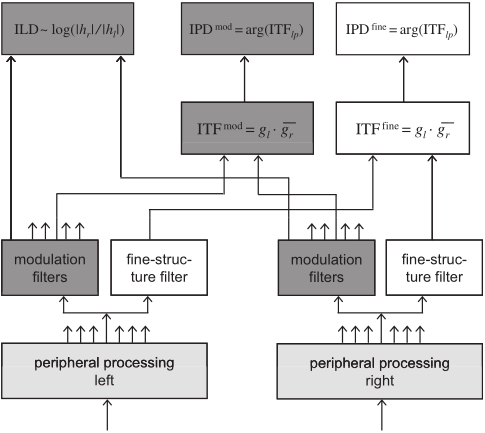
\includegraphics[width=\textwidth]{images/dietz_model_structure.png}
  \caption{Τα στάδια επεξεργασίας του ακουστικού μοντέλου. Η περιφερική επεξεργασία χωρίζει το σήμα εισόδου σε 23 ακουστικά φίλτρα ανά αυτί, και ακολουθείται από ανόρθωση ημίσεος κύματος, χαμηλοπερατό φιλτράρισμα και συμπίεση.}
  \label{fig:dietz_model_structure}
\end{figure}

\section{Λευκός Θόρυβος} \label{sec:white_noise}

Στην επεξεργασία σημάτων ο λευκός θόρυβος, είναι ένα τυχαίο σήμα, που έχει σταθερή ένταση σε όλες τις συχνότητες, δηλαδή σταθερή πυκνότητα φάσματος ισχύος \cite{Carter2009}. Ο όρος χρησιμοποιείται σε διάφορους τομείς, όπως η φυσική, οι τηλεπικοινωνίες και η ακουστική. Στον διακριτό χρόνο, ο λευκός θόρυβος είναι ένα διακριτό σήμα, του οποίου τα δείγματα αντιμετωπίζονται ως μία σειρά ασυσχέτιστων τυχαίων μεταβλητών, με μέση τιμή μηδέν, και πεπερασμένη απόκλιση. Εφόσον ο λευκός θόρυβος ακολουθεί την κατανομή που περιγράφεται στην εξίσωση \ref{eq 4}, αποκαλείται Additive White Gaussian Noise (AWGN). Αξίζει να σημειωθεί πως ο λευκός θόρυβος είναι μια καθαρά θεωρητική κατασκευή, από την άποψη ότι δεν υφίστανται σήματα με άπειρο εύρος ζώνης. Τυπικά ένα σήμα λευκού θορύβου έχει τη μορφή που φαίνεται στο Σχήμα \ref{fig:typical_white_noise}

\begin{CEquation}
    Z_n \sim N(0,W) \label{eq 4}
\end{CEquation}

\begin{figure}[h]
  \centering
  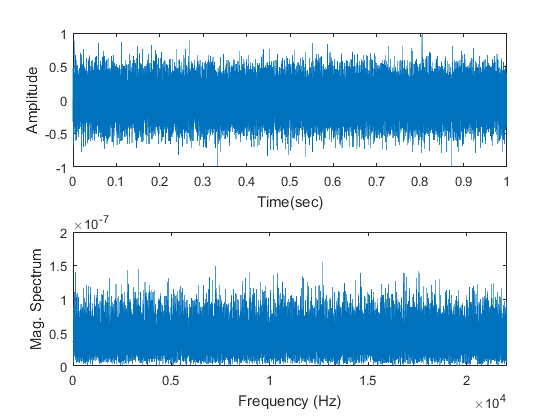
\includegraphics[width=\textwidth, height=8cm]{images/typical_white_noise.png}
  \caption{Τυπική μορφή σήματος λευκού θορύβου, στον χρόνο (Πάνω) και στη συχνότητα (Κάτω)}
  \label{fig:typical_white_noise}
\end{figure}

\section{Μηχανική Μάθηση}

Η ιδέα πίσω από τη μάθηση είναι ότι οι αισθήσεις δεν πρέπει να χρησιμοποιούνται απλώς για άμεση δράση, αλλά και για τη βελτίωση της ικανότητας ενός πράκτορα να ενεργεί στο μέλλον. Πράκτορας είναι οτιδήποτε μπορεί να θεωρηθεί ότι αντιλαμβάνεται το περιβάλλον του μέσω αισθητήρων, και επενεργεί σε αυτό το περιβάλλον μέσω μηχανισμών δράσης (Σχήμα \ref{fig:agent_environment_interaction}). Η μάθηση μπορεί να κυμαίνεται από την απλή απομνημόνευση των εμπειριών, μέχρι τη δημιουργία ολόκληρων επιστημονικών θεωριών. Εδώ περιγράφεται η επαγωγική μάθηση, κατά την οποία ένα σύστημα βελτιώνεται μέσω παρατηρήσεων \cite{Russell1994ArtificialIA}.

\begin{figure}[h]
  \centering
  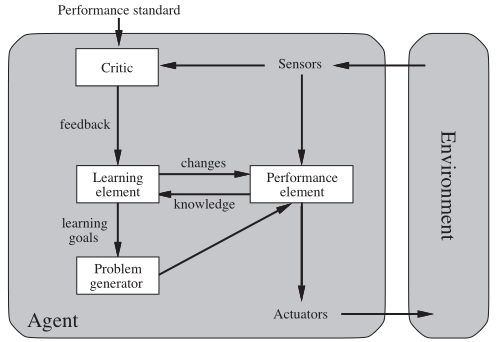
\includegraphics[width=\textwidth]{images/agent_environment_interaction.png}
  \caption{Αλληλεπίδραση πράκτορα με το περιβάλλον του}
  \label{fig:agent_environment_interaction}
\end{figure}

Ένας πράκτορας μπορεί να θεωρηθεί ότι περιλαμβάνει ένα στοιχείο εκτέλεσης, το οποίο αποφασίζει τι ενέργειες θα πραγματοποιήσει, και ένα στοιχείο μάθησης που τροποποιεί το στοιχείο εκτέλεσης έτσι ώστε να λαμβάνει καλύτερες αποφάσεις. Οι ερευνητές της μηχανικής μάθησης έχουν ανακαλύψει μια μεγάλη ποικιλία στοιχείων μάθησης. Για να γίνουν αυτά κατανοητά, είναι χρήσιμο να αποσαφηνιστεί το με ποιον τρόπο η σχεδίασή τους επηρεάζεται από το περιβάλλον στο οποίο θα εφαρμοστούν. Η σχεδίαση ενός στοιχείου μάθησης επηρεάζεται από τρία κύρια ζητήματα:
\begin{itemize}
    \item Ποιες συνιστώσες του στοιχείου εκτέλεσης πρέπει να μαθευτούν.
    \item Τι ανάδραση διατίθεται για τη μάθηση αυτών των συνιστωσών.
    \item Ποια αναπαράσταση χρησιμοποιείται για τις συνιστώσες.
\end{itemize}{}

Συνοπτικά \textbf{στοιχείο εκτέλεσης} είναι το στοιχείο του πράκτορα που είναι υπεύθυνο για εξωτερικές πράξεις και \textbf{στοιχείο μάθησης} το στοιχείο που είναι υπεύθυνο για την υλοποίηση βελτιώσεων στο σύστημα.

Ο \textit{τύπος της ανάδρασης} που διατίθεται για τη μάθηση είναι συνήθως ο πιο σημαντικός παράγοντας για τον προσδιορισμό της φύσης του μαθησιακού προβλήματος. Διακρίνονται τρεις περιπτώσεις: \textbf{μη επιβλεπόμενη μάθηση} (unsupervised learning), \textbf{επιβλεπόμενη μάθηση} (supervised learning) και \textbf{ενισχυτική μάθηση} (reinforcement learning).

\subsection{Μη επιβλεπόμενη μάθηση}
Το πρόβλημα της μη επιβλεπόμενης μάθησης περιλαμβάνει τη μάθηση προτύπων εισόδου χωρίς να παρέχονται συγκεκριμένες τιμές εξόδου. Δύο βασικές μέθοδοι είναι η \textit{ανάλυση σε κύριες συνιστώσες} (Principal Component Analysis - PCA) και η \textit{ανάλυση συστάδων} (cluster analysis). Χρησιμοποιείται ευρέως στην εκτίμηση πυκνοτήτων πιθανοτήτων (pdf) στη στατιστική.

\subsection{Ενισχυτική μάθηση}
Η ενισχυτική μάθηση είναι ένα πεδίο της μηχανικής μάθησης που ασχολείται με τον τρόπο που πράκτορες λογισμικού πρέπει να πάρουν αποφάσεις και να τις εκτελέσουν σε ένα περιβάλλον ώστε να μεγιστοποιήσουν κάποια ανταμοιβή. Όπως και η μη επιβλεπόμενη μάθηση, δεν χρειάζεται συγκεκριμένες τιμές εξόδου. Υλοποιείται τυπικά με την μορφή αλυσίδων αποφάσεων Markov

\subsection{Επιβλεπόμενη μάθηση}
H επιβλεπόμενη μάθηση είναι η διαδικασία της χαρτογράφησης μιας εισόδου σε μία έξοδο, με βάση \textit{labeled} δεδομένων εισόδου, που αποτελούνται από παραδείγματα εισόδου-εξόδου. Με αυτόν τον τρόπο, εκτιμάται μια συνάρτηση με βάση αυτά τα ζεύγη παραδειγμάτων. Κάθε παράδειγμα, είναι ένα ζεύγος, που αποτελείται από ένα αντικείμενο εισόδου, τυπικά ένα διάνυσμα, και μια επιθυμητή τιμή εξόδου. Σε ένα ιδανικό σενάριο, ο αλγόριθμος θα μπορεί να εκτιμήσει σωστά την επιθυμητή έξοδο από περιπτώσεις που δεν έχουν χρησιμοποιηθεί κατά την εκπαίδευση. Σε αυτή την κατηγορία αλγορίθμων μάθησης, εντάσσονται και τα Νευρωνικά Δίκτυα που θα απασχολήσουν αυτή την εργασία.

Πιο αυστηρά, ο στόχος της επιβλεπόμενης μάθησης είναι: Δοθέντος ενός \textbf{συνόλου εκπαίδευσης} Ν παραδειγμάτων ζευγών εισόδου-εξόδου: $$(x_1,y_1), (x_2,y_2), ... (x_N,y_N)$$ όπου κάθε $y_i$ δημιουργείται από μια άγνωστη συνάρτηση $y=f(x)$, να βρεθεί μια συνάρτηση $h$ που προσεγγίζει την $f$.

Όταν η έξοδος $y$ ανήκει σε ένα σύνολο πεπερασμένων τιμών, (λ.χ. ναι, όχι, ίσως) το πρόβλημα μάθησης λέγεται \textbf{ταξινόμηση} (classification). Όταν το $y$ είναι ένας πραγματικός αριθμός, το πρόβλημα λέγεται \textbf{regression}.

\begin{figure}[h]
  \centering
  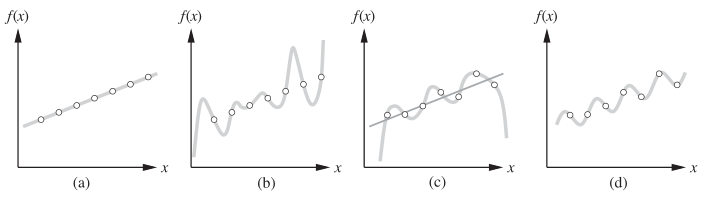
\includegraphics[width=\textwidth]{images/supervised_example_linear.png}
  \caption{Παραδείγματα ζευγών $(x,f(x))$ και υποθέσεις διαφορετικών βαθμών πολυωνύμου (a) 1ου βαθμού, (b) 7ου βαθμού. (c) Ένα διαφορετικό dataset και μια γραμμική εκτίμηση, (d) ημιτονοειδής εκτίμηση}
  \label{fig:supervised_example_linear}
\end{figure}

Στο Σχήμα \ref{fig:supervised_example_linear} φαίνεται ένα σύνηθες παράδειγμα, η προσαρμογή μιας καμπύλης σε ένα σύνολο ζευγών σημείων. Δεν είναι γνωστό ποια είναι η $f$ αλλά προσεγγίζεται με μια \textit{h} επιλεγμένη από τον χώρο υποθέσεων $\mathcal{H}$. Στο παράδειγμα αυτό είναι ένα σύνολο πολυωνύμων. 

Η επιβλεπόμενη μάθηση μπορεί να υλοποιηθεί επιλέγοντας την υπόθεση $h^*$ που είναι πιθανότερη με βάση τα δεδομένα:
\begin{CEquation}
\begin{split}
     h^* = \argmaxF_{h\subset\mathcal{H}} P(h|data)
     \label{eq:hypothesis_star}
\end{split}
\end{CEquation}


Η Εξίσωση \ref{eq:hypothesis_star} με βάση τον κανόνα του Bayes, μετασχηματίζεται στην Εξίσωση \ref{eq:hypothesis_star_bayes} και μπορεί κανείς να ισχυριστεί πως η εκ των προτέρων πιθανότητα $P(h)$ είναι μεγάλη για ένα πολυώνυμο μικρού βαθμού και χαμηλότερη για ένα πολυώνυμο μεγάλου βαθμού. Γενικότερα επιτρέπονται περίπλοκες ή \textit{παράξενες} προσεγγίσεις μόνο όταν κρίνεται ότι το απαιτούν τα δεδομένα, αλλά αποφεύγεται με τον να τους ανατίθεται χαμηλή πιθανότητα. Γενικά, αξίζει να σημειωθεί πως υπάρχει πάντα ένα tradeoff μεταξύ της εκφραστικότητας ενός χώρου υποθέσεων, και της πολυπλοκότητας της εύρεσης μιας καλής υπόθεσης μέσα σε αυτό το χώρο.

\begin{CEquation}
\begin{split}
     h^* = \argmaxF_{h\subset\mathcal{H}} P(data|h)P(h)
     \label{eq:hypothesis_star_bayes}
\end{split}
\end{CEquation}

\section{Νευρωνικά Δίκτυα}

Νευρωνικά Δίκτυα, ή με τον πιο δόκιμο όρο, Τεχνητά Νευρωνικά Δίκτυα (Artificial Neural Networks - ANN), είναι ένα σύνολο από τεχνητούς νευρώνες ή κόμβους \cite{Hopfield_1982}. Ουσιαστικά είναι υπολογιστικά συστήματα εμπνευσμένα από βιολογικά νευρωνικά δίκτυα που έχουν μελετηθεί σε εγκεφάλους διαφόρων ζώων \cite{Chen_2019}. Τα συστήματα αυτά 'μαθαίνουν' να εκτελούν συγκεκριμένο έργο λαμβάνοντας υπόψιν τους παραδείγματα, συνήθως χωρίς να είναι προγραμματισμένα με συγκεκριμένους κανόνες που αφορούν το εν λόγω έργο. Εκτελούν το έργο που τους ανατίθεται, χωρίς να έχουν πρότερη γνώση επί αυτού. 

\subsection{Νευρώνες} 

Ένα ANN βασίζεται σε μια συλλογή νευρώνων οι οποίοι μοντελοποιούν τους νευρώνες ενός βιολογικού εγκεφάλου. Κάθε σύνδεση, όπως οι συνάψεις στον εγκέφαλο, μπορεί να μεταδόσει σήματα στους άλλους νευρώνες. Ένας τεχνητός νευρώνας δέχεται το σήμα, το επεξεργάζεται και στη συνέχεια μεταβιβάζει το επεξεργασμένο σήμα στους νευρώνες με τους οποίους συνδέεται.

Αυστηρότερα, ένας νευρώνας είναι μια \textit{συνάρτηση}, και αποτελεί το δομικό στοιχείο ενός ANN. Δέχεται μία ή περισσότερες εισόδους, (που αντιπροσωπεύουν τα διεγερτικά μετασυναπτικά δυναμικά και τα ανασταλτικά μετασυναπτικά δυναμικά στους δενδρίτες των νευρώνων) τις προσθέτει και μεταδίδει μια έξοδο, (ή ενεργοποίηση που αντιπροσωπεύει το δυναμικό δράσης ενός βιολογικού νευρώνα που μεταδίδεται κατά μήκος του άξονά του). Η αντιστοίχηση φαίνεται στο Σχήμα \ref{fig:biological_neuron_artificial_neuron_cmp}. Συνήθως σε κάθε είσοδο ανατίθεται ένα βάρος και το άθροισμά τους δίνεται ως είσοδος σε μια μη γραμμική συνάρτηση που αποκαλείται \textbf{\textit{συνάρτηση ενεργοποίησης}} ή \textit{συνάρτηση μεταφοράς} του νευρώνα.

\begin{figure}[h]
  \centering
  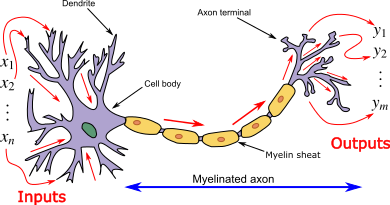
\includegraphics[width=\textwidth]{images/Neuron3.png}
  \caption{Νευρώνας και μυελινωμένος άξονας, με τη ροή του σήματος από τις εισόδους στους δενδρίτες στις εξόδους στον άξονα.}
  \label{fig:biological_neuron_artificial_neuron_cmp}
\end{figure}

\subsubsection{Βασική Δομή Νευρώνα}

Για έναν τεχνητό νευρώνα, έστω \textit{m + 1} είσοδοι με σήματα από $x_0$ μέχρι $x_m$. Η είσοδος σε έναν νευρώνα \textit{k} φαίνεται στην εξίσωση \ref{eq:kth_neuron_input}, όπου με \textit{φ} συμβολίζεται η συνάρτηση μεταφοράς ενώ η δομή ενός νευρώνα φαίνεται στο Σχήμα \ref{fig:artificial_neuron_math_model}.

\begin{CEquation}
\begin{split}
     y_k = \phi(\sum_{j=0}^mw_{kj}x_j)
     \label{eq:kth_neuron_input}
\end{split}
\end{CEquation}

\begin{figure}[h]
  \centering
  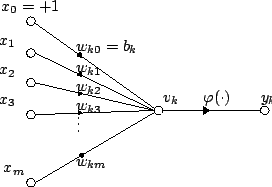
\includegraphics[width=8cm, height=6cm]{images/Artificial_neuron.png}
  \caption{Μαθηματικό μοντέλο ενός νευρώνα με bias στο $x_0 = 1$}
  \label{fig:artificial_neuron_math_model}
\end{figure}

\subsubsection{Συναρτήσεις ενεργοποίησης}

\begin{itemize}
    \item \textbf{Βηματική Συνάρτηση}: Η έξοδος αυτής της συνάρτησης είναι δυαδική και εξαρτάται από το αν η είσοδος ξεπερνά ή είναι ίση με ένα ορισμένο κατώφλι \textit{θ}. Εκτελεί μια διαίρεση του χώρου εισόδων με ένα υπερεπίπεδο. Είναι ιδιαίτερα χρήσιμη όταν εφαρμόζεται στο τελευταίο επίπεδο ενός ANN, που κάνει δυαδική συσταδοποίηση.
    \begin{CEquation}
    \begin{split}
         y = 
         \begin{cases}
         1 & \text{if}\;x\geq\theta\\
         0 & \text{if}\;x<\theta
         \end{cases}   
         \label{eq:step_function}
    \end{split}
    \end{CEquation}
    
    \item \textbf{Σιγμοειδής}: Μια μη-γραμμική συνάρτηση με παράγωγο που υπολογίζεται εύκολα, και κατ' επέκταση είναι υπολογιστικά απλή. Ένα παράδειγμα είναι η γνωστή logistic function:
    \begin{CEquation}
    \begin{split}
         y = \frac{e^x}{e^x + 1}  
         \label{eq:logistic_function}
    \end{split}
    \end{CEquation}
    
    \item \textbf{Συνάρτηση Ανόρθωσης}: Οι συναρτήσεις αυτές είναι γνωστές και ως συναρτήσεις ράμπας, και είναι το υπολογιστικό ανάλογο ενός ανορθωτή ημίσεος κύματος. Λέγονται επίσης Rectified Linear Units ή ReLU και ορίζονται ως εξής:
    \begin{CEquation}
    \begin{split}
         y = x^+ = \max{(0,x)}
         \label{eq:ReLU}
    \end{split}
    \end{CEquation}
    
\end{itemize}{}

\subsection{Οργάνωση}

Οι νευρώνες τυπικά είναι οργανωμένοι σε πολλά επίπεδα, ιδιαίτερα στην περίπτωση του deep learning. Το επίπεδο που δέχεται τα δεδομένα είναι το \textit{επίπεδο εισόδου}, ενώ το επίπεδο που δίνει το τελικό αποτέλεσμα είναι το \textit{επίπεδο εξόδου}. Μεταξύ τους μπορεί να υπάρχουν μηδέν ή περισσότερα \textit{κρυφά επίπεδα}. Τα επίπεδα μπορεί να είναι συνδεδεμένα με πολλούς τρόπους. Για παράδειγμα μπορεί να είναι \textit{πλήρως διασυνδεδεμένα}, με κάθε νευρώνα σε ένα επίπεδο να συνδέεται με όλους τους νευρώνες του επόμενου επιπέδου.

\subsubsection{Υπερπαράμετροι} \label{subsub:hyperparameters}

Μια υπερπαράμετρος είναι μια σταθερή παράμετρος της οποίας η τιμή ορίζεται πριν την εκκίνηση της διαδικασίας εκπαίδευσης. Τέτοιες παράμετροι είναι ο ρυθμός μάθησης (learning rate - LR), ή ο αριθμός των κρυφών επιπέδων.

\subsubsection{Backpropagation}

Το backpropagation είναι μια μέθοδος ρύθμισης των βαρών των συνάψεων για την διόρθωση των σφαλμάτων κατά την εκπαίδευση. Το σφάλμα πρακτικά 'μοιράζεται' σε όλες τις συνάψεις. Υπολογίζονται οι παράγωγοι των συναρτήσεων ενεργοποίησης ανάλογα με τα τωρινά βάρη, και ενημερώνονται αναλόγως με την μέθοδο βελτιστοποίησης που έχει επιλεχθεί. Σε αυτή την εργασία όλα τα μοντέλα χρησιμοποιούν τον Adam optimizer.

\subsubsection{Αρχιτεκτονικές}

Μία από τις αρχιτεκτονικές που χρησιμοποιείται σε αυτή την εργασία είναι ο πολυεπίπεδος Perceptron (Multilayered Perceptron - MLP). Η αρχιτεκτονική αυτή αποτελείται από τουλάχιστον τρία επίπεδα, ένα επίπεδο εισόδου, ένα επίπεδο εξόδου και τουλάχιστον ένα κρυφό επίπεδο, όλα πλήρως διασυνδεδεμένα μεταξύ τους. Η απλούστερη δομή (από την άποψη του αριθμού των επιπέδων) ενός MLP φαίνεται στο Σχήμα \ref{fig:multilayer-perceptron}.

\begin{figure}[h]
  \centering
  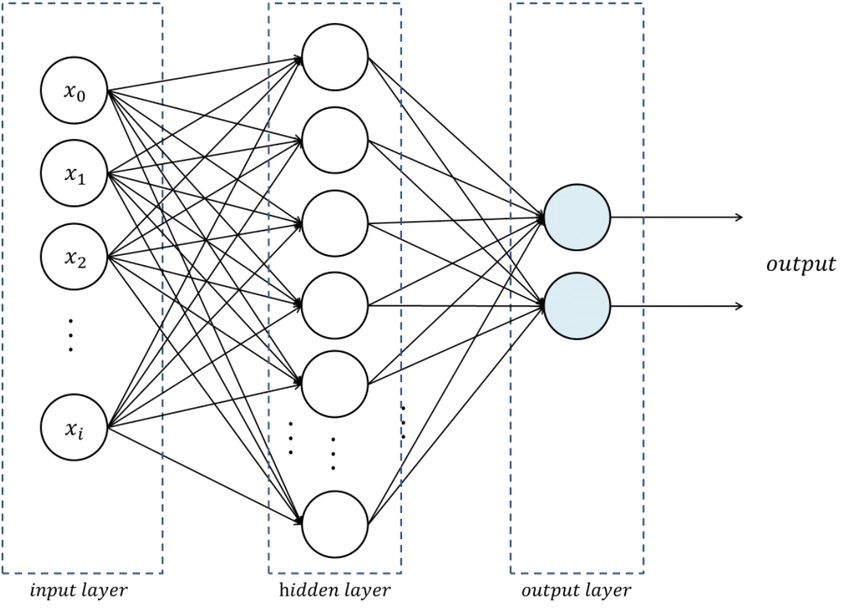
\includegraphics[width=\textwidth]{images/multilayer-perceptron.png}
  \caption{Η δομή του απλούστερου MLP.}
  \label{fig:multilayer-perceptron}
\end{figure}

Η δεύτερη αρχιτεκτονική που χρησιμοποιείται είναι αυτή των συνελικτικών δικτύων (Convolutional Neural Networks - CNNs). Η δομή αυτή είναι αρκετά πιο σύγχρονη από αυτή του MLP, και χρησιμοποιείται συχνά για την ανάλυση εικόνων και προβλήματα που αφορούν την υπολογιστική όραση. Αυστηρά, συνελικτικό δίκτυο είναι κάθε ANN που χρησιμοποιεί την πράξη της συνέλιξης. Στην πράξη, τα CNN, σε αντίθεση με τους MLP αντί να εκτολούν ένα γινόμενο πινάκων, χρησιμοποιούν συνέλιξη. Κάθε συνελικτικό επίπεδο, αποτελείται από έναν αριθμό φίλτρων που ορίζεται προτού ξεκινήσει η εκπαίδευση, όπως και οι διαστάσεις αυτών. Κάθε συνελικτικός νευρώνας επεξεργάζεται μόνο τα δεδομένα που είναι σε μια περιορισμένη υποπεριοχή της εξόδου του προηγούμενου επιπέδου. Μια τυπική δομή ενός CNN φαίνεται στο Σχήμα \ref{fig:convolutional-neural-network-architecture}. Οι λειτουργία των επιπέδων Pooling εξηγείται σε επόμενη ενότητα.

\begin{figure}[h]
  \centering
  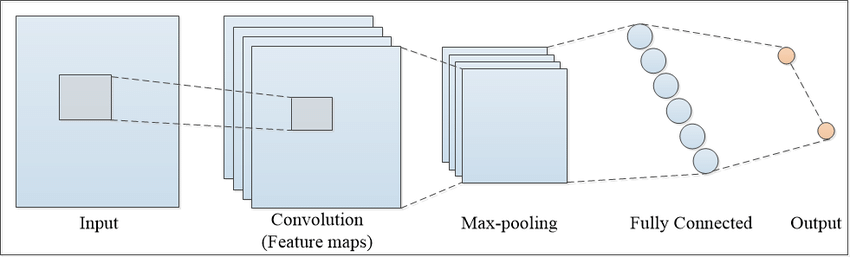
\includegraphics[width=\textwidth]{images/convolutional-neural-network-architecture-showing-a-feed-forward-pass-with-one.png}
  \caption{Η δομή ενός απλού CNN.}
  \label{fig:convolutional-neural-network-architecture}
\end{figure}
\newpage
\subsection{Συναρτήσεις Απώλειας}

Κάθε αλγόριθμος βελτιστοποίησης χρησιμοποιεί μια συνάρτηση για την \textit{αξιολόγηση} μιας πιθανής λύσης (π.χ. το σύνολο των βαρών στις συνάψεις ενός NN). Η συνάρτηση αυτή καλείται αντικειμενική συνάρτηση, και η βέλτιστη λύση είναι αυτή που ελαχιστοποιεί την αντικειμενική συνάρτηση σε προβλήματα ελαχιστοποίησης (ή το αντίθετο σε προβλήματα μεγιστοποίησης) \cite{Goodfellow2017}.

\subsubsection{Μέσο Απόλυτο Σφάλμα}
Το ΜΑΕ, είναι ένα μέτρο της διαφοράς μεταξύ δύο συνεχών μεταβλητών. Υποθέτοντας μεταβλητές Χ και Υ, οι οποίες είναι η πραγματική και η εκτιμώμενη τιμή αντίστοιχα, τότε για \textit{n} παρατηρήσεις το ΜΑΕ υπολογίζεται από την Εξίσωση \ref{eq:MAE}. Το ΜΑΕ έχει τις ίδιες μονάδες με τα δεδομένα που παρατηρούνται και πεδίο ορισμού $D = [0, +\infty)$. 

\begin{CEquation}
\begin{split}
     MAE = \frac{\sum_{i=1}^n|y_i-x_i|}{n}
     \label{eq:MAE}
\end{split}
\end{CEquation}


\subsubsection{Μέσο Τετραγωνικό Σφάλμα}
Το MSE ενός εκτιμητή, υπολογίζει τον μέσο όρο των τετραγώνων των σφαλμάτων, δηλαδή τον μέσο όρο των τετραγώνων των διαφορών της εκτιμώμενης τιμής από την πραγματική. Το MSE, είναι η δεύτερη ροπή (ως προς το 0) του σφάλματος, οπότε περιέχει τόσο την τυπική απόκλιση, δηλαδή το πόσο 'απλωμένες' είναι οι εκτιμήσεις, αλλά και  το \textit{bias}, δηλαδή το πόσο μακριά είναι η μέση εκτιμώμενη από την μέση πραγματική τιμή. Όπως η διακύμανση, έτσι και το MSE, έχει τις μονάδες των δεδομένων παρατήρησης υψωμένες στο τετράγωνο. Χρησιμοποιείται, όταν είναι ιδιαίτερα ανεπιθύμητα μεγάλα σφάλματα στον εκτιμητή, έχει πεδίο ορισμού το $D = [0, +\infty)$, και υπολογίζεται όπως φαίνεται στην εξίσωση \ref{eq:MSE}.

\begin{CEquation}
\begin{split}
     MSE = \frac{\sum_{i=1}^n|y_i-x_i|^2}{n}
     \label{eq:MSE}
\end{split}
\end{CEquation}

\subsubsection{Ρίζα Μέσου Τετραγωνικού Σφάλματος}
Το RMSE, αντιπροσωπεύει την τετραγωνική ρίζα της δεύτερης ροπής των διαφορών μεταξύ των εκτιμώμενων τιμών και των πραγματικών. Όπως και τα προαναφερθέντα μέτρα, είναι θετικά ορισμένο, με πεδίο ορισμού το $D = [0, +\infty)$. Συνδυάζει τα πλεονεκτήματα του MSE και του MAE, από την άποψη ότι 'τιμωρεί' περισσότερο τις μεγάλες αποκλίσεις από τις πραγματικές τιμές, αλλά είναι ταυτόχρονα πιο εύκολα ερμηνεύσιμο, όπως το MAE, αφού είναι και αυτό σε γραμμική κλίμακα. Υπολογίζεται όπως φαίνεται στην Εξίσωση \ref{eq:RMSE}

\begin{CEquation}
\begin{split}
     RMSE = \sqrt{\frac{\sum_{i=1}^n|y_i-x_i|^2}{n}}
     \label{eq:RMSE}
\end{split}
\end{CEquation}
